\chapter{Lemon Cake}
\label{ch:Lemoncake}
\index{dessert}
\index{cake}
\index{lemon}

\marginnote{
    \textbf{Makes 1 Pyrex dish} \\
    Prep time: 30 minutes + overnight chilling\\
    Cook time: 0 minutes \\
    \vspace*{\baselineskip}

    3 packets Lemon pie mix, Dr. Oetker Shirriff \\
    1 can of peaches \\
    1 tsp cornstarch \\
    1 packet tea cookies, Goglu \\
    \vspace*{\baselineskip}
    
    \textbf{Ingredients for decoration} \\
    Nutriwhip, or Coolwhip, or Heavy whipping cream \\
    Maraschino cherries \\
    Slivered almonds
}

\marginalfigure{monanteras/images/Shirriff Lemon pie mix.png}{Shirriff Lemon pie mix}{fig:Lemoncake}

% \begin{figure}
%   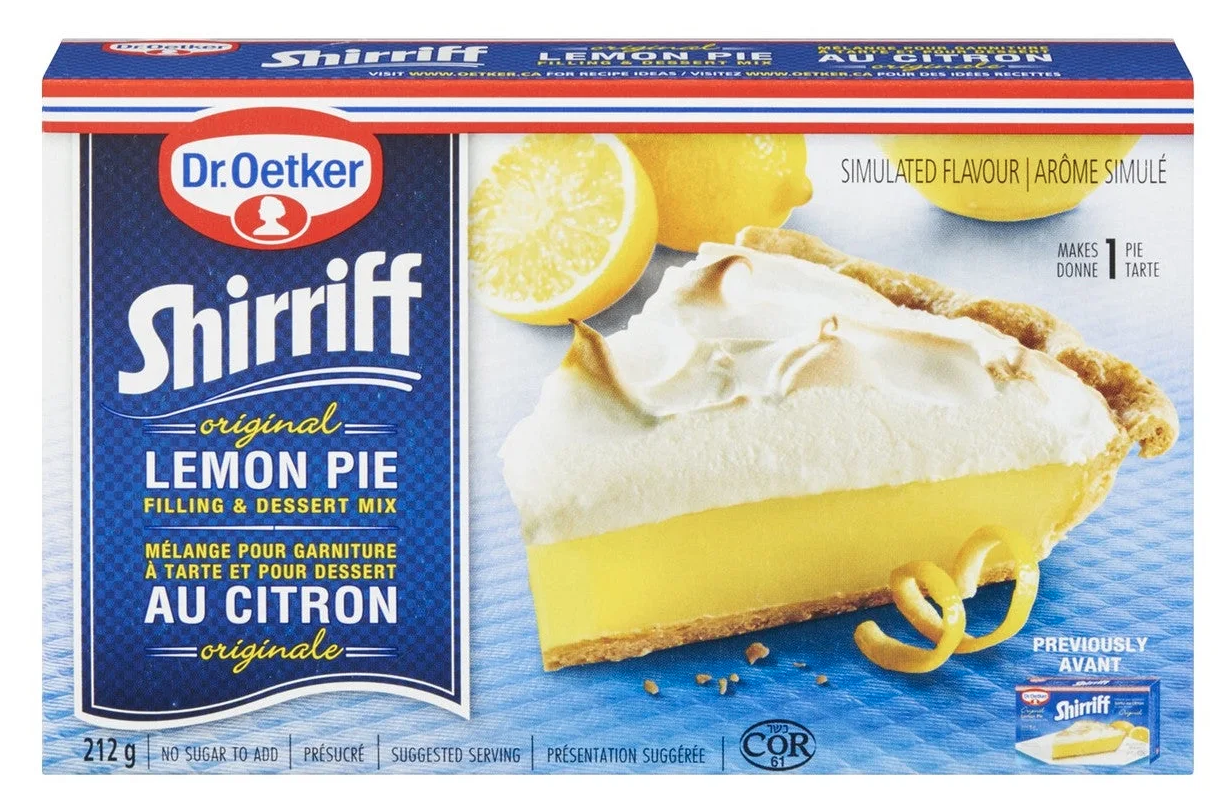
\includegraphics[width=60mm]{monanteras/images/Shirriff Lemon pie mix.png}
%   \caption{Shirriff Lemon pie mix}
% \end{figure}
%
\textit{Lemon no-bake cake with peaches}

Family member: Grandma Eleni

\newthought{I have} vague memories of eating this cake during summertime on my grandma's balcony, when it was really hot and sunny. The sourness and refreshing lemon was perfect during summertime.

\begin{enumerate}
    \item Dip Goglu cookies in the juice of the canned peaches, and line them at the bottom of a large rectangular glass Pyrex.
    \item Prepare the 3 packets of Lemon pie mix following the directions. Pour the lemon mix on top of the cookies.
    \item In a small pot, warm the peach juice. Once it is boiling, add 1 tsp cornstarch and whisk until smoothe and thickened. Pour it evenly on top of the lemon curd.
    \item Whip the Nutriwhip (or Heavy cream if using) and spread it evenly on top. Add enough to create a nice 1-2 inch layer and create waves with a spoon or small spatula. 
    \item Decorate with maraschino cherries, slivered almonds, and some peaches if desired. Keep in fridge until ready to serve.
\end{enumerate}

\captionfigure{monanteras/images/Lemon cake.jpg}{Grandma Eleni with her cake}{fig:Lemoncake_2}
\captionfigure{monanteras/images/Lemon cake 2.jpg}{Celebrating Grandma's 84th birthday}{fig:Lemoncake_3}

% \begin{figure}
%   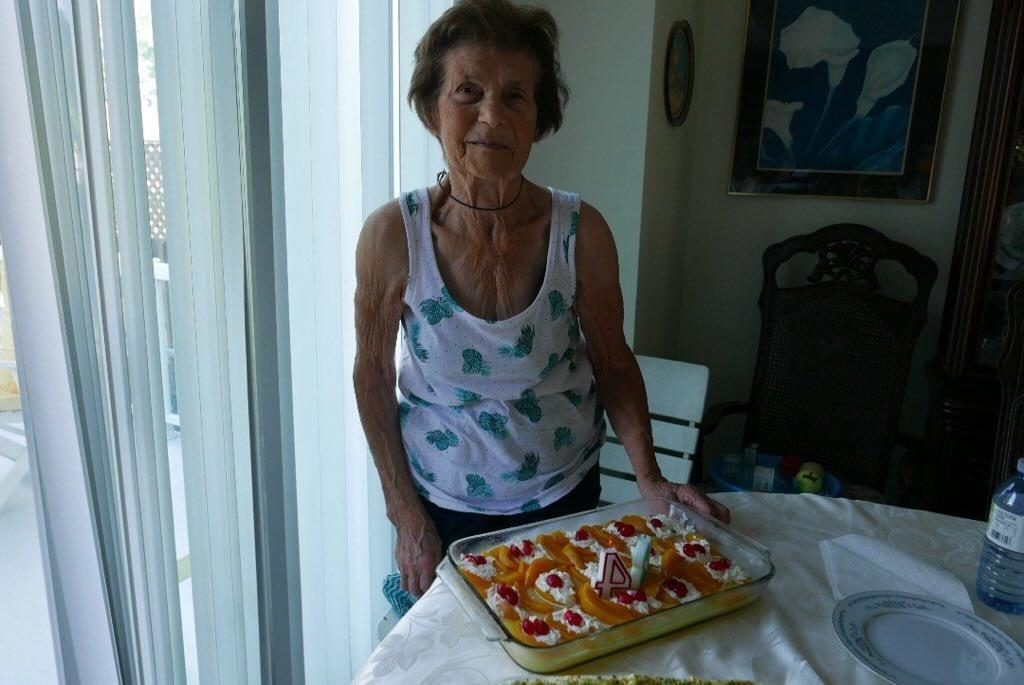
\includegraphics[width=80mm]{monanteras/images/Lemon cake.jpg}
%     \caption{Celebrating Grandma's 84th birthday}
% \end{figure}
% \begin{figure}
%   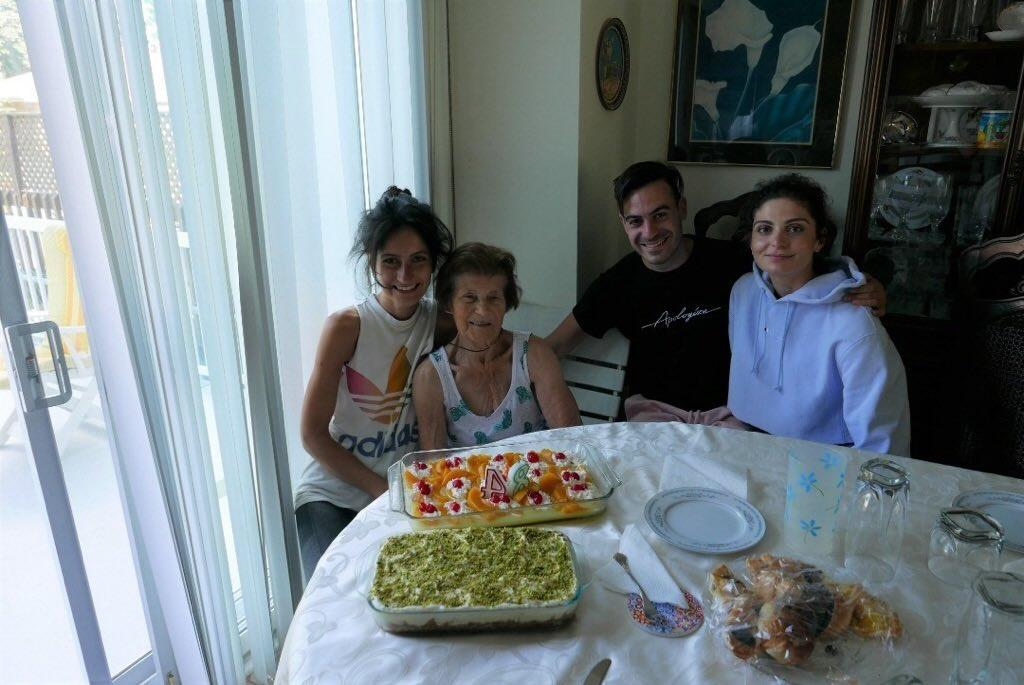
\includegraphics[width=80mm]{monanteras/images/Lemon cake 2.jpg}
% \end{figure}
